% ---------------------------------------------------------------------- %
% TODO
%
% - [ ] spelling and capitalization of
%   - [ ] ocropy, OCRopus, <del>OCRopy</del>
%   - [ ] kraken, tesseract
%   - [ ] calamari (OCR)
%   - [ ] common API
% - [ ] Table 1: Update GitHub Stars, SLOC and date checked
% - [ ] Add URLs to models
% - [ ] Add citations to OCR-D MP
% - [ ] revisit abstract
% - [ ] Submit :)
%
% ----------------------------------------------------------------------


\documentclass[conference]{IEEEtran}
\IEEEoverridecommandlockouts
\usepackage{cite}
\usepackage{amsmath,amssymb,amsfonts}
\usepackage{algorithmic}
\usepackage{graphicx}
\usepackage{rotating}
\usepackage{cleveref}
\usepackage{hyperref}
\usepackage[utf8]{inputenc}
\usepackage{textcomp}
\usepackage{xcolor}
\usepackage{multirow}
\begin{document}

\title{
okralact - a multi-engine Open Source OCR training system \\
\thanks{This work was partially supported by the Deutsche Forschungsgemeinschaft (DFG) - Project number 274863866}
}

\author{%
\IEEEauthorblockN{1\textsuperscript{st} Konstantin Baierer}
\IEEEauthorblockA{\textit{Staatsbibliothek zu Berlin} - \\
\textit{Preu\ss{}ischer Kulturbesitz} \\
konstantin.baierer@sbb.spk-berlin.de}
\and
\IEEEauthorblockN{2\textsuperscript{nd} Rui Dong}
\IEEEauthorblockA{\textit{Khoury College of Computer Sciences} \\
\textit{Northeastern University}\\
dongrui@ccs.neu.edu}
\and
\IEEEauthorblockN{3\textsuperscript{rd} Clemens Neudecker}
\IEEEauthorblockA{\textit{Staatsbibliothek zu Berlin} - \\
\textit{Preu\ss{}ischer Kulturbesitz} \\
clemens.neudecker@sbb.spk-berlin.de}
}

\maketitle

% CN: Here is the call for papers:
% https://www.primaresearch.org/hip2019/callForPapers. For the purposes of HIP,
% it is important to stress the context of _historical_ documents. We can (and
% should, I will write sth) introduce the "problem" of historical document
% processing first like: a) what are the challenges of historical documents,
% why do we require more tailored solutions b) the possibilities of NNs and
% training, thus being able to train models for historical documents that can
% outperform off-the-shelf general OCR classifiers c) the lack of an ecosystem
% for Open Source OCR model generation due to (why?) i) bad usability/docs
% toolchain for training and their diversity and ii) lack of ground
% truth/standardization...you know this much better than me. This is the
% introduction. Then we proceed with a short discussion of Open OCR, and what
% the pros/cons of the selected algorithms are and why it is beneficial to be
% able to train all of them from one "system" - here we can e.g. argue for
% better evaluation/testing/replicability. Now the main part comes with the
% description of okralact... To close, it is important to provide a clear
% perspective again as to how this work will contribute to solving the
% challenges of historic documents from the introduction.

\begin{abstract}

Optical character recognition (OCR) of historical documents has
been significantly more difficult than OCR of modern texts
largely due to idiosyncrasies and wide variability of font,
layout, language, orthography of printed texts before ca.
1850. However, common OCR engines are optimized towards
supporting the widest possible set of modern text ("OmniFont
OCR") with little or no facilities for the user to adapt the
engine. Since OCR technologies began embracing deep neural
networks, various Free Software OCR engines are now available
that can in principle be adapted to different types of
documents by training specific models from ground truth (GT).
What these engines offer in terms of implementation finesse,
they lack in interoperability and standardization. To overcome
this, we developed okralact, a set of specifications and a
prototypical implementation of an engine-agnostic system for
training Open Source OCR engines like tesseract, ocropus,
kraken or calamari. We briefly compare these engines, describe
the specifications and functionality of okralact and outline
how a turn-key system for adapting Open Source OCR engines can
contribute to better OCR of historical documents and to the
wider OCR ecosystem.

\end{abstract}

\begin{IEEEkeywords}
OCR, ocropus, kraken, calamari, tesseract
\end{IEEEkeywords}

\section{Introduction}


Advances in deep learning have been a game-changer for image
processing, document layout analysis and text recognition, key components of optical
character recognition (OCR). Text recognition technology in
particular has seen a paradigm-shift, away from a combination of character
segmentation and pattern-based detection, towards
segmentation-free recognition based on trained neural networks
(NN).
% Since training from GT is so essential for the process, all NN-based OCR engines
% offer tools to train new models. However the usability of these training tools
% varies wildly. Different engines have different assumptions n the kind of input
% data they expect, the kind of hardware they are run on and employ slightly different
% terminology. The trained models are engine-specific, sometime even to a specific
% version of an engine and in most cases, it is very difficult to assess what
% kind of data a model was trained on after the fact.
%Any NN-based approach involves two steps: Training a model based on manually
%annotated ground truth (GT) and applying this model to data, in the case of
%OCR to recognize the text in images.

Most of the state-of-the-art OCR engines apply a hybrid recurrent convolutional
neural network combined with a connectionist temporal classification (CTC)
\cite{graves2006connectionist} layer as the OCR model. Deep convolutional
neural networks (CNN) \cite{krizhevsky2012imagenet} are added as the bottom
layers to extract hierarchical location-invariant features from the raw images
\cite{wick2018improving}. Recurrent neural networks (RNN)
\cite{mikolov2010recurrent}, which are effective in capturing the dependencies
in temporal sequences, are then added on top of the CNN layers to extract
sequential image representations. The CTC layer allows the text recognition
model to be trained on pairs of images and ground truth text without explicitly
aligning between them. It both saves the efforts of segmenting the images into
characters and avoids the possible errors introduced in this process.

In the particular context of historical documents and Fraktur fonts, e.g.
\cite{breuel2013high} have applied RNN with LSTM for OCR and obtained 
competitive accuracy when compared to ABBYY FineReader, tesseract or OCRopus. 
An additional benefit that comes with the application of LSTM is the omission 
of a specific language model or dictionary, both of which are typically sparse 
for historical language, without trading off recognition accuracy.\cite{ul2013can}

%Any NN-based approach involves two steps: Training a model based on manually
%annotated ground truth (GT) and applying this model to data, in the case of
%OCR to recognize the text in images.

However, these NN-based OCR engines vary wildly in their design
assumptions, e.g., the format of the input data, the hardware
requirements, as well as the set of adjustable parameters for
building and training an OCR model. For example, some engines can
only be run on CPU devices while others can tap into the
computation power of GPU devices. Some allow users to build their
own neural networks while others have a fixed model structure. The
trained models are engine-specific, sometimes even down to a specific
version of the engine and in most cases, it is very difficult to
assess what kind of data a model was trained on after the fact. All
of this has prevented the wider adoption and provision of NN-based OCR models
for historical printed documents.

To overcome these obstacles to adoption, we propose
\textit{okralact}, a flexible set of specifications and a software
prototype to harmonize the input data, parameterization and
provenance tracking of training different OCR engines.
\textit{Okralact} is developed within the context of
OCR-D\footnote{http://ocr-d.de/eng}, a composition of a
coordination and several module projects established with support
from Deutsche Forschungsgemeinschaft (German Research Foundation,
DFG). OCR-D has the aim to examine available technologies for OCR and via the 
definition of standards and best-practices in combination with the adaptation and development of state-of-the-art NN-based methods contribute to improving the OCR process for mass-digitization of 
printed historical material.\cite{neudecker2019datech}  

% TODO

% CN: Outline of the remaining paper - check when final! 

The remainder of this paper is divided into four sections. Section
II provides an overview of the currently most prominent Free
Software OCR engines and discusses their training features and models 
in more depth. Section III introduces \textit{okralact} with its
specification and the prototype implementation. We conclude by 
outlining remaining challenges and future work in section IV. 

\section{Open Source OCR}

There have been various Free Software projects that implement NN technologies
for OCR. For the scope of this work, we only consider the four most prominent projects: tesseract, ocropus, kraken and calamari, all of which are released under the Apache License 2.0.

%\begin{table}[b]
%\begin{tabular}{llll}
%\hline
%Engine    & Main Developer     & Stack                      & Development \\ \hline
%OCRopus   & Tom Breuel         & Python                     & stale       \\
%kraken    & Benjamin Kiessling & Python, Torch              & active      \\
%Calamari  & Christoph Wick     & Python, Tensorflow         & active      \\
%tesseract & Ray Smith          & C++                        & active
%\end{tabular}
%\caption{Basic properties of Open Source OCR engines}
%\label{tab:basic}
%\end{table}

\begin{table}[b]
\begin{tabular}{lllll}
\hline
Engine    & Contributors & First Release & GitHub Stars & SLOC \\ \hline
OCRopus   & 28           & 2010          & 2557         & 4996 \\
kraken    & 10           & 2015          & 146          & 4065 \\
Calamari  & 7            & 2018          & 299          & 6116 \\
tesseract & 102          & 1985          & 27135        & 143251 \\

\end{tabular}
\caption{Software metrics of selected Open Source OCR engines as of 2019-05-22}
\label{tab:stats}
\end{table}

\subsection{tesseract}

tesseract \cite{4376991} was one of the first Free Software OCR
engines \cite{Rice1995TheFA} and remains one of the oldest OCR engines still in
development. Consistently helmed by Ray Smith, tesseract has gone
through various iterations and partial rewrites and changing
ownership. Open Source since 2005 and sponsored by Google since
2006, tesseract is the most well-known and most widely used Open
Source OCR engine (c.f. Table \ref{tab:stats}).

While earlier versions of tesseract did contain training facilities, 
these had severe limitations and required cumbersome data preparation and
character-based training. Attempts in training tesseract for historical documents, e.g.
by the IMPACT \cite{PSNC} and eMOP \cite{doi:10.1093/llc/fqv062} projects, did not yield 
the desired improvements in OCR accuracy.

With the first alpha of version 4.0.0 released in 2016, tesseract introduced a trainable
engine based on LSTM NN.\cite{smith2016tesseract} While still a very involved, multi-step process, the
improved accuracy and fine-tuning to specific corpora outweighs the effort.
There have been activities to streamline the training process, e.g.
ocrd-train\footnote{\url{https://github.com/OCR-D/ocrd-train}.} implements a training workflow for
tesseract 4 as a Makefile.

\subsection{OCRopus}

The brainchild of Thomas Breuel and first released in 2007, OCRopus
\cite{breuel} was initially a set of tools around OCR based on
tesseract. With the release of the Python implementation ocropy in
2010, OCRopus revolutionized OCR by adopting
Long-Short-Term-Memory (LSTM). OCRopus bundled a set of rudimentary but
usable command line tools not only to train and apply models but
also to preprocess images (binarization, deskewing, layout analysis),
evaluate recognition results and a basic user interface to produce
GT data. Breuel has since moved on to create clstm, a better
performing LSTM implementation \cite{DBLP:conf/icdar/Breuel17}, and
ocropy2, a rewrite of OCRopus based on CUDA and the PyTorch Deep
Learning framework \cite{DBLP:conf/icdar/Breuel17} but neither has
yet reached the same traction in the Free Software community as the
original Python version.

Ocrocis is a noteable augmentation of OCRopus, providing best practices and
additional scripts and automation solutions for training.\cite{springmann2015ocrocis}

% TODO: Mention Ocrocis?

\subsection{kraken}

kraken \cite{DBLP:journals/corr/RomanovMSK17} started out as a fork of ocropy
by Benjamin Kiessling in 2015 to rectify a number of implementation and usability
issues while preserving (mostly) functional equivalence. While retaining many of
the algorithms around OCR, the actual recognition engine has been based on the
Torch machine learning framework since version 2.0 and can not reasonably be
considered a fork of ocropy anymore. kraken has been having a particular impact
on OCR of Arabic and is the technical foundation of the Open Islamic Texts
Initiative \cite{miller_romanov_savant_2018}.


\subsection{calamari}

Christoph Wick has been developing the Calamari
\cite{DBLP:journals/corr/abs-1807-02004} OCR engine since 2018, based on the
codebases of ocropy and kraken but backed by the TensorFlow machine learning
framework. Calamari also added advanced features such as n-fold training and
voting algorithms and is used as the main component of the OCR4all
framework.\footnote{\url{https://github.com/OCR4all}.}

\subsection{Feature comparison}

% The goal of \textit{okralact} is to wrap all the engines into a common

Different OCR engines display different design features in terms of the
technical details of implementation and the interfaces provided to the users.

\subsubsection{Implementation}

Tesseract is implemented in C++ while the
other three engines are all written in Python. Tesseract and ocropy
implement the neural networks as well as the inference from scratch without
utilizing any existing deep learning libraries. Kraken uses PyTorch as the
deep learning backend. Calamari allows using different deep learning backends,
though currently only the TensorFlow backend is implemented.

%\subsubsection*{Library Dependencies}

\subsubsection{Hardware Requirements}

Both kraken and calamari support GPU training, which offers significant
improvements with regard to computation speed compared to training on CPU devices.

% kba: Rui, which engines benefit from GPU in recognition?

\subsubsection{Model Parameters}

Table~\ref{tab:model_param1} illustrates that different OCR engines provide
different levels of freedom for the users to design their own neural network
structures. OCRopus does not support CNN as the feature extractor for raw
images. The raw image features are directly fed into the LSTM layers. It only
allows users to choose whether to use bidirectional or unidirectional LSTM
layer and the size of hidden states. The number of LSTM layers is fixed.
Tesseract, kraken and Calamari provide more modeling options to the user. They
allow users to add arbitrary numbers of CNN, pooling, dropout and RNN
layers. All three engines support user specified kernel size and output size in
CNN layer, but tesseract and kraken also provide additional options for
activation functions.

% kba: Rui can we substantiate these features with citations? "Pooling" can mean
% a lot of things in different contexts, e.g.

\begin{table}[bt]
\begin{tabular}{llllll}
\hline
Layers                   & Parameters   & OCRopus              & kraken   & Calamari & tesseract \\ \hline
% CNN Layer& & NA & Yes & Yes & Yes  \\
\multirow{ 3}{*}{CNN}    & kernel size  & \multirow{3}{*}{NA} & \checkmark        & \checkmark        & \checkmark         \\
                         & activation   &                      & \checkmark        & -        & \checkmark         \\
                         & output size  &                      & \checkmark        & \checkmark        & \checkmark         \\ \hline
\multirow{2}{*}{Pooling} & kernel size  & \multirow{2}{*}{NA}  & \checkmark        & \checkmark        & \checkmark         \\
                         & stride size  &                      & \checkmark        & -        & \checkmark         \\ \hline
\multirow{2}{*}{Dropout} & probability  & \multirow{2}{*}{NA}  & \checkmark        & \checkmark        & \checkmark         \\
                         & dimension    &                      & \checkmark        & -        & \checkmark         \\ \hline
\multirow{2}{*}{RNN}     & output size  & \checkmark                    & \checkmark        & \checkmark        & \checkmark         \\
                         & direction    & \checkmark                    & \checkmark        & -        & \checkmark         \\
                         & dynamic cell & lstm                 & lstm/gru & lstm     & lstm/gru  \\
                         & time axis    & -                    & \checkmark        & -        & \checkmark         \\ \hline
Output                   & output size  & -                    & \checkmark        & -        & \checkmark         \\
\end{tabular}
\caption{Model Design Options for Open Source OCR engines.}
\label{tab:model_param1}
\end{table}

\subsubsection{Training Parameters}

The four OCR engines provide different levels of flexibility to fine-tune training
parameters such as the learning rate, which optimizer to use or whether to stop early,
as summarized in Table~\ref{tab:training_options}. For different
optimizers, different OCR engines also provide different ways to adjust
optimizer parameters. All four engines allow the user to specify how long the
model should be trained in terms of maximum number of training samples, epochs
or iterations. Kraken, Calamari and tesseract also support early stopping,
i.e., stopping training earlier than the specified ending point, when the model
performance satisfies some given conditions. For example, kraken supports early
stopping when the model performance improvement is not significant any more. Tesseract
stops training when the error rate is lower than a user specified target error
rate. Calamari stops training when the model performance is continuously
getting worse.

\begin{table}[bt]
\begin{tabular}{llllll}
\hline
Parameters                     &         & OCRopus & kraken & Calamari & tesseract \\ \hline
% CNN Layer                      &         & NA      & Yes    & Yes      & Yes       \\
\multirow{2}{*}{Learning Rate} & overall & -       & \checkmark      & \checkmark        & \checkmark         \\
                               & layer   & -       & -      & -        & \checkmark         \\
\hline
Optimizer                      &         & -       & \checkmark      & -        & \checkmark         \\ \hline
Early Stop                     &         & -       & \checkmark      & \checkmark        & \checkmark         \\
%\hline
% Maximum &           & lines & epoches                 & iterations               & iterations   \\
%         & condition &       & performance not         & performance continuously & error rate   \\
%         &           &       & significantly improving & getting worse            & small enough \\ \hline
\end{tabular}
\caption{Training Options for Open Source OCR engines.}
\label{tab:training_options}
\end{table}

\subsubsection{Fine Tuning}

All four engines provide a user interface for fine-tuning an
existing model with new training data. Ocropy only allows
continued training of an existing model with new data samples,
while the other three engines also allow the user to modify the
structure of an existing model. Users can cut off the top of the 
network at a given layer and append a new model structure after it.
For example, when a user wants to train an OCR model for a new
language which shares lots of characters with the existing model,
the bottom CNN layers can be reused to extract similar image
features.


\subsubsection{Tooling / User Interfaces}

All examined OCR engines provide basic user interfaces to
train OCR models, although they vary in the set of adjustable
parameters and ease of use. Calamari and kraken, due their lineage,
provide some tools similar to ocropy or advise to use ocropy's tools
directly. The ocropy codebase is not developed further hence the interfaces
are frozen in the state of ca. 2015, also to avoid breaking legacy OCR
workflows. Both kraken and calamari significantly improve the command
line interfaces. While kraken allows for elegant and terse calls by
removing configurability of obsolete or little-used features, Calamari
exposes as much of the power to the user, resulting in a long list
of parameters.

% kba: not very well phrased but you know

Training tesseract is
significantly more complex than training the other three engines. OCRopus,
kraken and calamari all require a single command line call to train
a model, while the process with tesseract is more involved.
For example, tesseract requires the users
to generate bounding boxes for each text line although it does not
really need individual character coordinates. The character set is then
explicitly generated from all the bounding boxes files with the
command ``\textit{unicharset\_extractor}''. The training data are
provided to the training interface via ``lstmf'' files, where each
file is serialized document data containing an image and the
corresponding GT text. These files are generated via the
command ``\textit{tesseract}''. Then a traineddata file is generated
to obtain all the information it needs on the language to be
learned via ``\textit{combine\_lang\_model}'' command. Finally,
command ``\textit{lstmtraining}'' is used to train an OCR model with
the traineddata file and the list of lstmf files as input.

\subsubsection{Standard models}

A well-engineered OCR engine is only the technical foundation for
good recognition results. How accurately a particular model recognizes text
in a particular document crucially depends on how the model was trained. In
an ideal world of unlimited resources, technically proficient domain experts
would transcribe corpus- or even document-specific GT and use a system such as
\textit{okralact} or the training facilities of individual engines to train
tailor-made models for maximum recognition accuracy. In reality, due to lack of
resources to transcribe GT and train models as well as the technical
challenges involved, the availability and quality of ready-to-use models is 
essential to the quality of an OCR engine perceived by the bulk of users.

Tesseract has the widest range of pretrained models available of the engines
supported by okralact. Trained on synthetic data, there are models available
for a wide variety of languages and scripts, including Fraktur. Since the shift
to NN-based recognition, two tiers of models are available, tessdata\_best and
tessdata\_fast, with the latter trading off accuracy for recognition speed. Since
training is so complex, there are few community-provided models available at this
moment, if any.

% citation required for the details on tesseract model GT

The default model provided by OCRopus author Tom Breuel has been trained on
both synthetic and real GT and has been widely used in both ocropy and kraken.
Breuel also offers a model for recognition of Fraktur. The OCRopus community
has been developing models for Old French, Polytonic Greek and Japanese. Uwe
Springmann has developed a methodology for training document-specific models
for OCRopus and shared some of his models for historical documents.

Kraken integrates the widest variety of models and model formats,
supporting not only ocropy and clstm models but also a more efficient
protobuf-based encoding of ocropy models and, since version 2.0, CoreML-encoded
models. As part of the architecture, models can be loaded from a GitHub-based
model repository, offering models for Arabic, Polytonic Greek and German Fraktur.

% https://github.com/mittagessen/kraken-models

Calamari supports only its proprietary model format but uses the same approach
to model distribution as kraken, offering a GitHub repository with pretrained
models, mostly targeted towards German in both Antiqua and Fraktur scripts.

% https://github.com/Calamari-OCR/calamari_models

Tesseract is the only project that publishes the GT the standard models are
trained on. In general, provenance information on GT, model structure and training parameters is missing for the standard models of all engines.
The kraken models are described by a very basic JSON metadata format but not
deeply enough to recreate the model. Adapting the specifications outlined
in section \ref{sec:specs}, e.g. by training with the okralact implementation
described in \ref{sec:prototype}, full provenance information can be retained,
making the models more widely usable and sustainable.


\section{okralact}


% TODO: be more specific
\textit{Okralact} is both a set of specifications and a prototype
implementation for harmonizing the input data, parameterization and
provenance tracking of training different OCR engines.

\subsection{Specifications}
\label{sec:specs}

\textit{Okralact} is an integral part of the OCR-D project that has been
consolidating specifications and Open Source software around OCR
with a focus on enabling mass full text digitization of historical
documents.\footnote{\url{https://ocr-d.github.io}.} As with the
OCR-D project proper, the primary focus of \textit{okralact} is to develop
specifications, technical documentation about the different engines
and their parameterization. These specifications are made
actionable in a prototype training infrastructure (c.f.
\ref{sec:prototype}) but are developed with different usage
scenarios and implementations as well as the upstream engine
developers in mind.

First, we propose a container format for bundling OCR GT data.
While OCR engines expect GT in the form of line-wise image-text
tuples and supported file formats, encodings, file structure and
naming vary from engine to engine. The engines operate on image and
text data exclusively without the need for layout information.
Therefore, no engine currently supports any of the common OCR file
formats (ALTO, hOCR, PAGE-XML) as input. We aim to change this by
reusing as input format the OCRD-ZIP GT container format developed
within OCR-D.\footnote{\url{https://ocr-d.github.io/ocrd_zip}.}
\cite{boenig2019datech} This will allow users to apply advanced
tools for GT creation, such as e.g.  PRImA Research Labs' Aletheia
\cite{clausner2011aletheia}.

Secondly, we compared the parameterization of the tools and
identified a set of common parameters that are equivalent across
engines, yet may differ slightly in their usage or terminology.
Beyond this common API, there are various configuration options and
parameters that are unique per engine. We gathered this information
in a JSON Schema document that defines the common API and
engine-specific parameters in a machine-actionable
form.\footnote{\url{https://ocr-d.github.io/gt-profile.yaml}.} The
schema can then be used to validate input configurations to the
training engine or to generate documentation such as help pages,
user interface hints and auto-completion.

% CN: Here is the first time BagIt gets mentioned we may need a ref
Lastly, we look at how trained models are distributed and
define another BagIt profile for describing trained models. This
format allows bundling not only the (engine-specific) models but
also the configuration that was used to train it and optionally the
GT that the model was based upon. 
% CN: rephrase next sentence
This allows broader reuse of models
since it contains the provenance of the model in terms of GT used,
parameterization, intermediary evaluation results and log files.

% * OCRD-ZIP GT format (shortly)
% * JSON schema for parameters / common API
% * https://github.com/OCR-D/spec/pull/105/files
%     * Drop the line GT part
%     * Clean up evaluation

\begin{figure*}[ht!]
    \begin{center}
        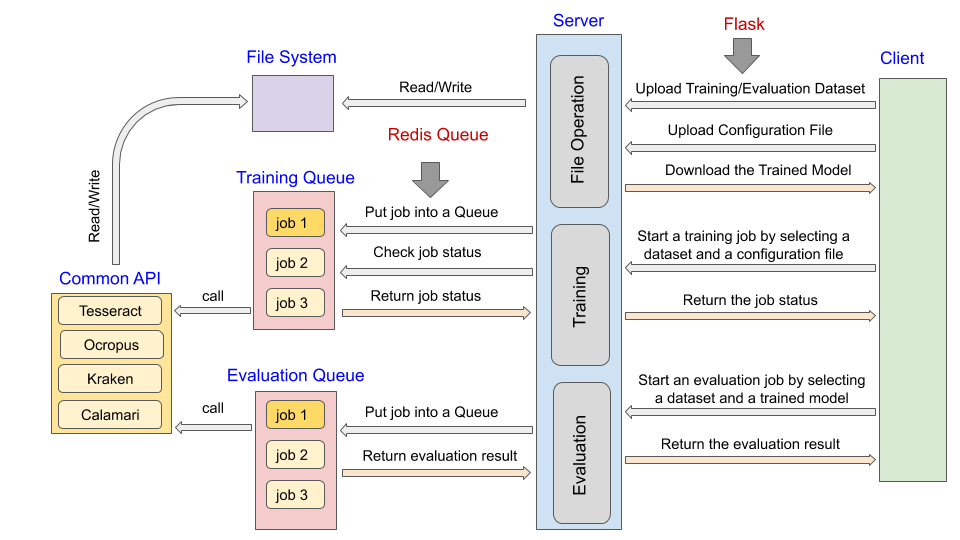
\includegraphics[width=1\linewidth]{Figures/Framework.png}
    \end{center}
    \caption{Framework of the \textit{okralact} system.}
    \label{fig:framework}
\end{figure*}

\subsection{Prototype}
\label{sec:prototype}

As shown in Figure \ref{fig:framework}, \textit{okralact} is a client/server
architecture application. The interactions between the client nodes and the
server are implemented using Flask, a lightweight web application framework.
Users can upload training or evaluation datasets and configuration files
specifying the OCR engine(s) and parameters to be used. The user can also
submit a request of training an OCR model with the selected dataset and
configuration file. After the job is submitted, the user can check the job
progress. Once the training of a model has completed, it can be downloaded.
The user can also submit an evaluation request with an evaluation dataset and
a selected model and receive evaluation report for the OCR results. 

% kba: Rui what does the user receive for the evaluation request?
% CN: Looks like currently Levenshtein distance is calculated, for
% future work bag-of-words might be a useful addition (segmentation
% errors)

% kba: We should briefly explain how we run the evaluation (not rely on the numbers by the engines but regularly recognize with snapshot models, calculate adapted levenshtein for CER, considering WER or BOW WER).

Since training and evaluation are both long-running process, HTTP communication must be asynchronous,
i.e., all the training or evaluation
jobs submitted to the server are handled in the background by Redis Queue,
a Python library built on top of Redis that
executes the work outside an HTTP request-response cycle. It puts job
requests into the queue of a given worker, which serves in
first-in-first-out order. When a job gets run, it performs a call to the common
API for different OCR engines to interpret the configuration files into the
training or evaluation command for the specified OCR engine. 

It is worth noting that \textit{okralact} has its own component of generating the evaluation report. Different engines provide evaluation report with different level of details. kraken provides very detailed report about the character error rate and the confusion matrix, while  
% kba: Rui what about evaluation jobs?


\section{Conclusion and Future Work}

With the current state of \textit{okralact}, it is possible to describe the
training process in a standardized way and specify the most important aspects 
of engine configuration with the common API, the engine-specific features with custom
parameters. The implementation supports basic training with all four engines
but does not yet support advanced features like n-fold training or training
continuation.

% kba: Rui?

% * [X] Adapt diagram \url{https://docs.google.com/presentation/d/1jyV7pWGkIgtIrc9uJ5jbUwNthOk0JSUgT_tA2QudwkA/edit#slide=id.p}
% * [X] Describe HTTP API
%   * [X] Draft a `/evaluation` endpoint taking evaluation config, model, groundTruth and %returning measures like CER, WER ...

% Expanded Common API by engine developers cooperating

Though we largely succeeded in harmonizing the majority of engine APIs into the
okralact common API, there still remain many engine-specific parameters. Some
features, like Calamari's n-fold training or tesseract's advanced language
modelling, are so engine-specific that forcing them into the common API would
be over-engineering. For those features, users can augment the common API
with engine-specific parameters, enabling power users to use the full range of
engine capabilities while requiring next to no knowledge of engine implementation
by less technically inclined users.

However, we hope to encourage engine developers and
users to discussions about unified terminology, data types and exchange 
formats that can help improve engine interoperability and therefore 
make \textit{okralact} even more accessible to non-expert users by extending
the range of the common API still.

% Cleanly defined evaluation measures necessary (no more ISRI or character-counting CER)

% Furthermore, there is a sore lack of easy to use tools with well
% defined measures for the evaluation of OCR. Traditionally, the
% character error rate (CER) and to a lesser extent word error rate
% (WER) have been the ratios to measure accuracy. However, these
% measures require perfect GT and results can be misleading for
% breakdowns in preprocessing such as segmentation errors or
% technical flaws in model preparation such as characters not part
% of the encoding.
% see prototype

% CN: At least within IAPR, CER/WER is still the most prominent and
% undisputed metric. One could perhaps argue for consideration of
% ReadingOrder in the evaluation, for necessary normalizations of
% encodings, how to deal with (and which) stopwords, asf. - but I
% am not really aware of any concerted efforts in this direction?
% TBH, the whole claim made here that evaluation methods and
% metrics are a challenge in this context is not yet entirely clear
% to me?

% More flexible choice of input data (multiple works, individual lines from individual pages etc.)

% Integration of training workflow and recognition workflows

Lastly, we aim for a better integration of training and
recognition workflows. As \textit{okralact} is part of the OCR-D
ecosphere, which has been developing components of a full-stack
OCR workflow, including image preprocessing, layout detection, font
detection, layout classification, recognition and language-model
post-processing, we intend to integrate \textit{okralact} into the
OCR-D specification and reference implementation. This will enable
users to pick and choose the best Free Software implementations for
the hole gamut of text recognition needs.

% kba: Plug our module projects by citing papers here.


%\section*{References}

% Please number citations consecutively within brackets \cite{b1}. The
% sentence punctuation follows the bracket \cite{b2}. Refer simply to the reference
% number, as in \cite{IEEEexample:bluebookbook} ---do not use ``Ref. \cite{b3}'' or ``reference \cite{b3}'' except at
% the beginning of a sentence: ``Reference \cite{b3} was the first $\ldots$''
%
% Number footnotes separately in superscripts. Place the actual footnote at
% the bottom of the column in which it was cited. Do not put footnotes in the
% abstract or reference list. Use letters for table footnotes.
%
% Unless there are six authors or more give all authors' names; do not use
% ``et al.''. Papers that have not been published, even if they have been
% submitted for publication, should be cited as ``unpublished'' \cite{b4}. Papers
% that have been accepted for publication should be cited as ``in press'' \cite{b5}.
% Capitalize only the first word in a paper title, except for proper nouns and
% element symbols.
%
% For papers published in translation journals, please give the English
% citation first, followed by the original foreign-language citation \cite{b6}.

\bibliographystyle{IEEEtran}
\bibliography{bibliography}

\end{document}
